\begin{figure*}[h]
    \centering
    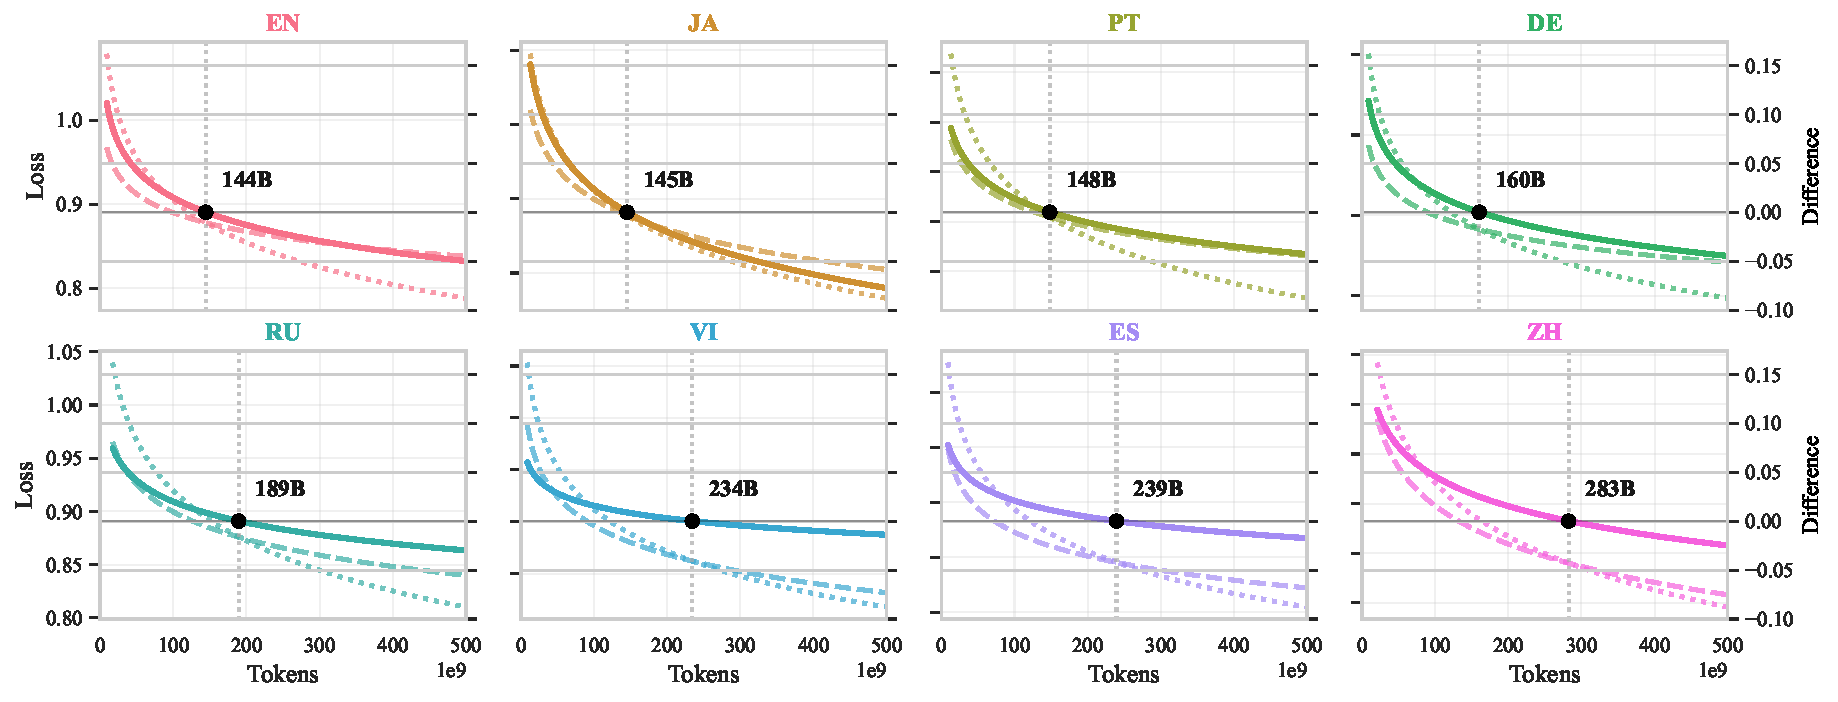
\includegraphics[width=\textwidth]{figures/finetune/pretrain_vs_finetune_lc_grid.pdf}
    \vspace{-4mm}
    \caption{For eight languages, we plot the loss curves for 2B parameter models pretraining monolingually from scratch (\textbf{···}), finetuning monolingually from the \unimax{} base model (\textbf{- - -}), and the difference between these losses (\textbf{---}).
    We annotate the number of tokens at which the pretrained loss becomes better than the finetuning loss.
    The difference between the interpolated pretraining curve and finetuning curve.
    When the loss difference reaches zero, pretraining from scratch has surpassed finetuning using equal compute.
    \textbf{Depending on the token (or compute) budget, it is usually more effective to finetune a multilingual checkpoint if there are $<144B$ tokens, and pretrain from scratch if the budget accommodates $\ge283B$ tokens.} 
    }
    \label{fig:pretrain_vs_finetune_learning_curves}
    % \vspace{-4mm}
\end{figure*}

% \vspace{-1mm}
\section{Pretrain or Finetune?}
\label{sec:finetune}
% \vspace{-1mm}

\noindent\textbf{Research Question:} \emph{When training a model for target language $t$, is it more effective to pretrain from scratch, or finetune a general-purpose massively multilingual checkpoint?}

\begin{wrapfigure}{L}{0.5\textwidth}
    \centering
    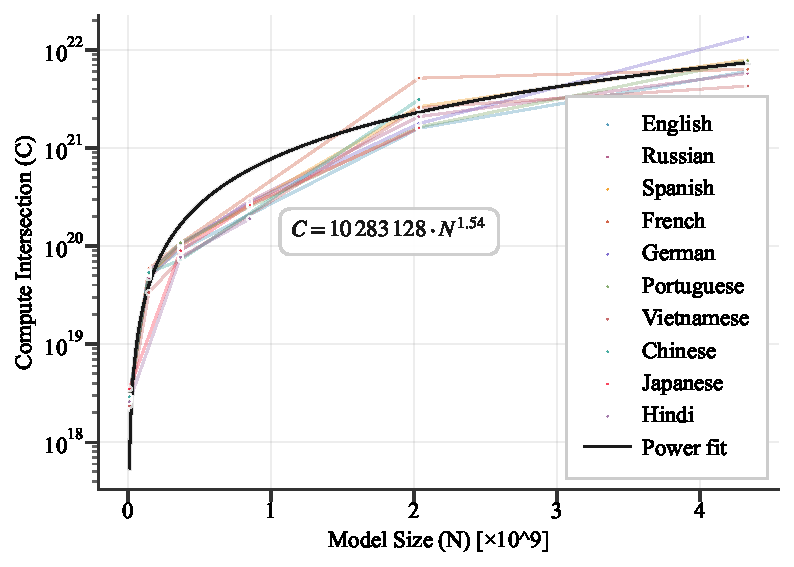
\includegraphics[width=0.48\textwidth]{figures/finetune/tails_intersection.pdf}
    % \vspace{-4mm}
    \caption{In terms of $N$, we model the compute budget $C$ required for a model pretrained from scratch to outperform the model finetuned from the generic \unimax{} multilingual checkpoint. 
    \textbf{We estimate this relationship as $C=10283128\,\times\,N^{1.65}$. }
    }
    \label{fig:modelsize_vs_finetune_intersection}
    \vspace{-4mm}
\end{wrapfigure}

Prior scaling law work focuses on compute efficiency with respect to pretraining from scratch.
However, in reality, practitioners who aim to optimize for a target language $t$ may have the option to start from multilingual public checkpoints or pretrain one multilingual checkpoint to serve as the starting point for many downstream models.
Consider a practitioner with a compute budget $C$. 
In \Cref{fig:pretrain_vs_finetune_learning_curves}, we plot the interpolated loss curves for the model pretrained from scratch, the model finetuned from a checkpoint, and the difference between these losses, for several languages.
We find that while the warm-started finetuned model performs better at first, pretraining from scratch eventually surpasses its performance after $144B\,-\,283B$ tokens, depending on the language.
Note that we leave the reason for these convergence differences to future work, without a clear hypothesis.
Though English pretraining converges the fastest, it is also allocated a 5\% sampling rate within \unimax{}, whereas each of the other languages are allocated 1.4\%.


From the number of training tokens $D$ we can also infer the inflection point which decides whether it is more computationally efficient ($C=6ND$) to pretrain from scratch or finetune from the multilingual checkpoint.
Using our range of model size experiments, we can estimate a best fit power law in \Cref{fig:modelsize_vs_finetune_intersection}, relating $N$ to $C$.
We find $log(C)=1113708\,\times\,N^{1.65}$ to hold consistently across languages.
For simplicity, we choose not to account for data repetition in this model.
Practitioners may use this to estimate whether pretraining or finetuning will yield greater performance for their compute budget.
% Notably, we can also estimate the pareto frontier loss across pretraining and finetuning, for each language, as illustrated in \Cref{finetune_intersection_pareto}.
Note one limitation to consider: not all multilingual base models are trained with the same mixture or for sufficiently long---and these factors would impact the pretrain vs finetuning intersection points. We choose a widely used \unimax{} mixture trained for 1B tokens~\citep{chung2023unimax}. We believe this is a useful heuristic, with reasonable assumptions, to determine the optimal choice between pretraining and finetuning for a given compute budget.

